\subsection{Drug model}
In order to simulate the effect of Propofol and Remifentanil on the depth of hypnosis the standard pharmacokinetic-pharmacodynamic (PK-PD) structure is used. The PK part models the distribution of drugs in the body using a compartment-model resulting in two decoupled LTI system, one for each drug. The outputs of this models are two effect-site drug concentrations which can be linked to the hypnotic effect by the PD part using a surface model response to model the synergic effect between both drugs. The final, model can be expressed by the following equation:

\begin{equation}
\begin{array}{ll}
        \dot{x}(t) = A x(t) + B u(t)\\
        y(t) = f(x(t)) + w(t),
    \end{array}
\label{eq:model}
\end{equation}

where $x(t) \in \mathbb{R} ^8$ represent the concentration of drugs inside the different compartments, particularly $x_4(t)$ and $x_8(t)$ are respectively the Propofol and Remifentanil effect-site concentration. $u(t)=\begin{pmatrix}
u_p(t) & u_r(t) \\
\end{pmatrix}^\top$ are the Propofol and Remifentanil drug rates injected into the patient blood. $f$ is the surface model function that can be describe by the following equation:
\begin{equation}
	f(x(t)) = BIS_0 + E_{max} \frac{I(t)^\gamma}{1 + I(t)^\gamma},
\end{equation}

where $BIS_0$ is the initial BIS, $E_{max}$ the maximum effect of combined drugs, $\gamma$ the slope coefficient of the Hill curve and $U(t)$ the interaction term defined by:

\begin{equation}
I(t) = \frac{x_{4}(t)}{C_{50p}} + \frac{x_{8}(t)}{C_{50r}}.
\end{equation}

$C_{50p}$ and $C_{50r}$ are the Propofol and Remifentanil half-effect concentrations for BIS ({\em i.e.} the concentrations to achieve half the effect of the drugs).

Finally $w(t)$ is the measurement noise. In the paper, a white noise filtered by a second order low pass filter with a cut-off frequency of 0.03 Hz is used to replicate real condition.
\medskip

In the simulation, the parameters of \cite{eleveldPharmacokineticPharmacodynamicModel2018} and \cite{eleveldAllometricModelRemifentanil2017} are used respectively for Propofol and Remifentanil PK model. For the PD model the parameters from \cite{bouillonPharmacodynamicInteractionPropofol2004} are implemented. \\
To perform simulation as close to the reality as possible uncertainties are added to the parameters. Particularly, each parameter is following a log-normal distribution (parameters of the distribution are specified in the previously cited paper) and a realization of the distribution is used for each patient. Simulation are done using the Python Anesthesia Simulator \cite{aubouin-pairaultPASPythonAnesthesia2023}.

\subsection{Drug rates tunning}

During the total intravenous anesthesia, Propofol and Remifentanil are dosed using Target Concentration Infusion (TCI) pumps. Those pumps include the nominal PK models, the anesthetist can select a concentration target and the pumps will compute and inject the drug to reach the target thanks to the model in an open loop matter. At the end the anesthetist is tunning the concentration target to reach the desired level of hypnosis.
\medskip


In order to recreate this scheme of control, TCI control algorithm \cite{shaferAlgorithmsRapidlyAchieve1992} have been reproduced. To mimic the comportment of the anesthesiologist the following rules have been coded:
\begin{itemize}
\item At the beginning the target concentration are set to $u_p = 4 \mu g/mL$ and $u_r = 4 ng/mL$.
\item A control period is randomly drawn for each patient and each drugs between 3 and 7 minutes. At each end of the period, the concentration target of the given drugs is updated as follows:
\begin{itemize}
	\item If $55<BIS$ the target is increased by 0.5.
	\item If $40<BIS$ the target is decreased by 0.5.
\end{itemize}
In addition, for Propofol only:
\begin{itemize}
	\item If $BIS>60$ the target is increased by 1.
	\item If $BIS<40$ the target is decreased by 1.
\end{itemize}
\end{itemize}

An example of the resulting control is exposed Fig~\ref{fig:test_control}.

\begin{figure}
\center
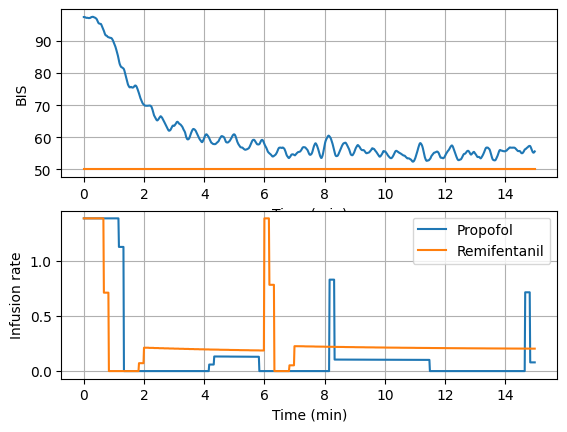
\includegraphics[width=0.7\textwidth]{images/test_control.png}
\caption{Results of the control algorithm for a single random patient.}
\label{fig:test_control}
\end{figure}

\subsection{Characteristics of the database}

The final databased includes induction (15 minutes) simulation files for 500 different patients with a sampling time of one second. Patients characteristic have been randomly chosen using uniform distribution (age $\in [18,70]$ height $ \in [150, 190]$, weight $\in[50,100]$, and gender $\in \{0,1\}$). Each file includes all the signals from the simulator, particularly the BIS values and the drug rates over time are available. An additional file includes the parameters of each patient. Figures~\ref{fig:BIS_data}-\ref{fig:concent_data} expose the results of the simulations.

\begin{minipage}[c]{.46\linewidth}
    \begin{figure} [H]
        \centering
        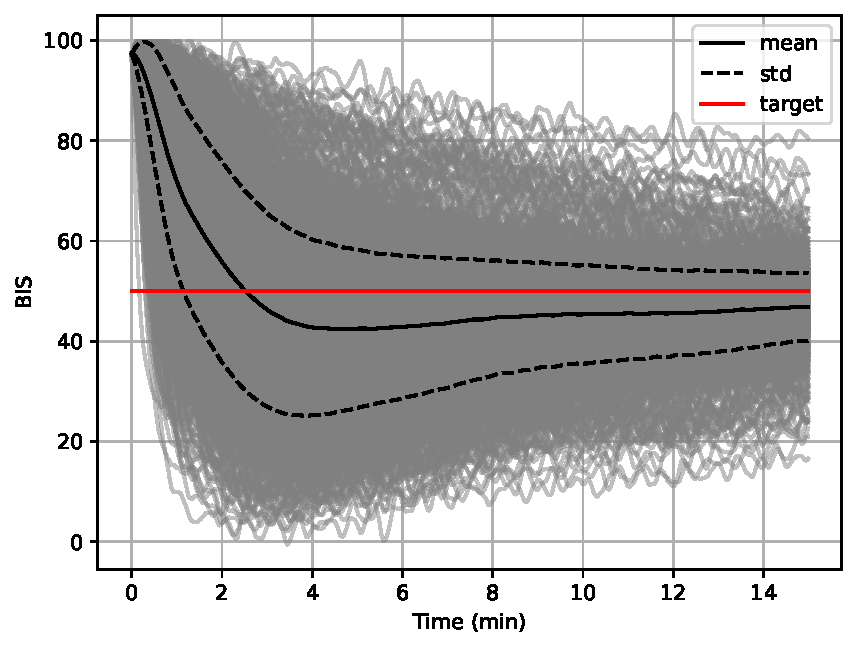
\includegraphics[width=0.8\textwidth]{images/BIS_data.pdf}
        \caption{BIS trajectory for all the simulations.}
        \label{fig:BIS_data}
    \end{figure}
\end{minipage}
\begin{minipage}[c]{.46\linewidth}
    \begin{figure} [H]
        \centering
        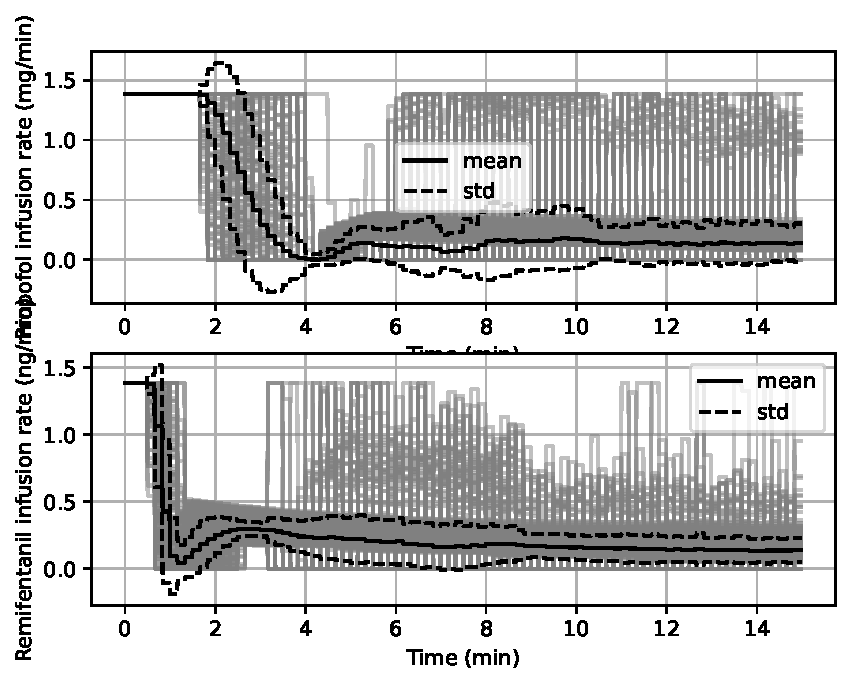
\includegraphics[width=0.8\textwidth]{images/input_data.pdf}
        \caption{Drug input rates for all the simulations.}
        \label{fig:input_data}
    \end{figure}
\end{minipage}
\begin{figure} [H]
\centering
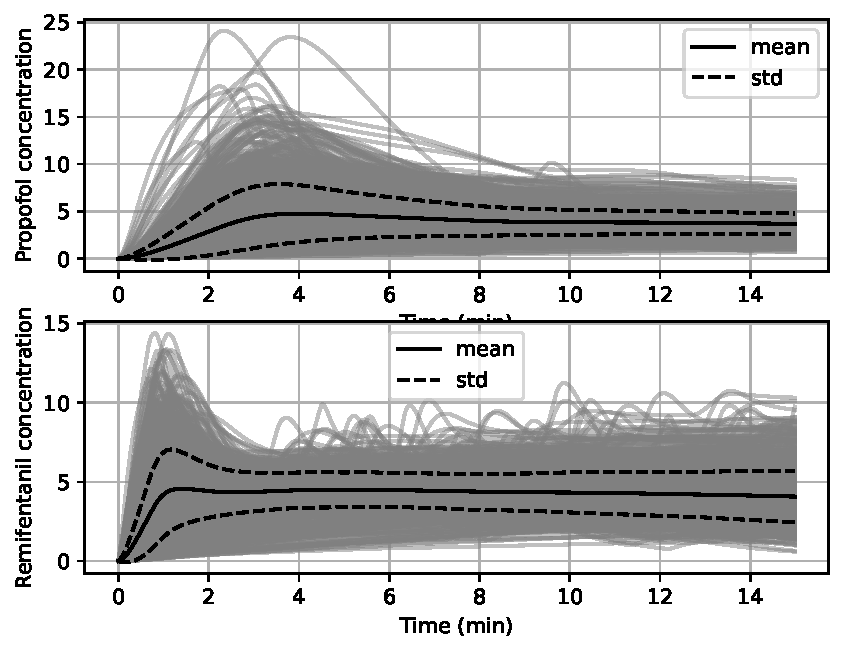
\includegraphics[width=0.5\textwidth]{images/concentration_data.pdf}
\caption{Drug effect-site concentration for all the simulations.}
\label{fig:concent_data}
\end{figure}